\documentclass[tikz]{standalone}
\usetikzlibrary{shapes.callouts}
\tikzset{
    level/.style = {
        ultra thick,
        black,
    },
    connect/.style = {
        dashed,
        red
    },
    notice/.style = {
        draw,
        rectangle callout,
        callout relative pointer={#1}
    },
    label/.style = {
        text width=2cm
    }
}
\begin{document}
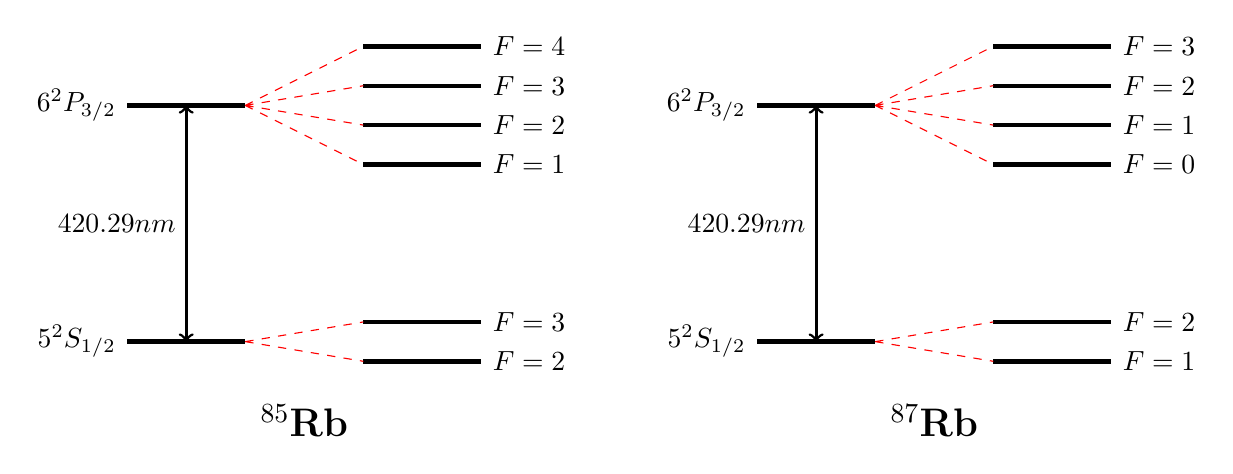
\begin{tikzpicture}
    % Draw all levels
    \newcommand\XA{0}
    \newcommand\XB{8}
    %RB85
    \node at (\XA+2.25,-1) {\Large\bf $^{85}$Rb};
    %6P3/2 
    \draw[level] (\XA+0,3) node[left] {$6 ^{2}P_{3/2}$} (\XA+0,3) -- (\XA+1.5,3);
    \draw[level] (\XA+3,3.75) -- (\XA+4.5,3.75) node[right] {$F=4$};
    \draw[level] (\XA+3,3.25) -- (\XA+4.5,3.25) node[right] {$F=3$};
    \draw[level] (\XA+3,2.75) -- (\XA+4.5,2.75) node[right] {$F=2$};
    \draw[level] (\XA+3,2.25) -- (\XA+4.5,2.25) node[right] {$F=1$};

    \draw[connect] (\XA+1.5,3) -- (\XA+3,3.75) (\XA+1.5,3) -- (\XA+3,3.25) 
                    (\XA+1.5,3) -- (\XA+3,2.75) (\XA+1.5,3) -- (\XA+3,2.25);

    %5S1/2
    \draw[level] (\XA+0,0) node[left] {$5 ^{2}S_{1/2}$} (\XA+0,0) -- (\XA+1.5,0);
    \draw[level] (\XA+3,0.25) -- (\XA+4.5,0.25) node[right] {$F=3$};
    \draw[level] (\XA+3,-0.25) -- (\XA+4.5,-0.25) node[right] {$F=2$};

    \draw[connect] (\XA+1.5,0) -- (\XA+3,-0.25) (\XA+1.5,0) -- (\XA+3,0.25);
    
    %Arrow
    \draw[<->,line width=1] (\XA+0.75,0) -- (\XA+0.75,3) node[midway, left]{$420.29nm$};

    %RB87
    \node at (\XB+2.25,-1) {\Large\bf $^{87}$Rb};
    %6P3/2 
    \draw[level] (\XB+0,3) node[left] {$6 ^{2}P_{3/2}$} (\XB+0,3) -- (\XB+1.5,3);
    \draw[level] (\XB+3,3.75) -- (\XB+4.5,3.75) node[right] {$F=3$};
    \draw[level] (\XB+3,3.25) -- (\XB+4.5,3.25) node[right] {$F=2$};
    \draw[level] (\XB+3,2.75) -- (\XB+4.5,2.75) node[right] {$F=1$};
    \draw[level] (\XB+3,2.25) -- (\XB+4.5,2.25) node[right] {$F=0$};

    \draw[connect] (\XB+1.5,3) -- (\XB+3,3.75) (\XB+1.5,3) -- (\XB+3,3.25) 
                    (\XB+1.5,3) -- (\XB+3,2.75) (\XB+1.5,3) -- (\XB+3,2.25);

    %5S1/2
    \draw[level] (\XB+0,0) node[left] {$5 ^{2}S_{1/2}$} (\XB+0,0) -- (\XB+1.5,0);
    \draw[level] (\XB+3,0.25) -- (\XB+4.5,0.25) node[right] {$F=2$};
    \draw[level] (\XB+3,-0.25) -- (\XB+4.5,-0.25) node[right] {$F=1$};

    \draw[connect] (\XB+1.5,0) -- (\XB+3,-0.25) (\XB+1.5,0) -- (\XB+3,0.25);
    
    %Arrow
    \draw[<->,line width=1] (\XB+0.75,0) -- (\XB+0.75,3) node[midway, left]{$420.29nm$};

    
\end{tikzpicture}
\end{document}